\label{informal-chapter}
\section{A New Methodology for Security Verification}
\label{informal-methodology}

In this chapter, we discuss the main ideas and challenges for defining 
and proving \emph{secure specifications}, and for propagating
security from a specification to its implementation. The fundamental
idea is to connect everything using what we call an 
\emph{observation function}. Recalling Figure~\ref{fig:methodology}, 
we use the observation function to (1) define a security policy at 
the specification level,
(2) formalize and prove noninterference with respect to the policy,
(3) define the observable whole-execution behaviors of a program,
and finally (4) automatically propagate security from a
high-level specification to a low-level implementation.

Intuitively, the observation function represents which parts of 
a program state are observable (i.e., low security) to each principal.
The observation being made by a principal does not actually have to be a 
portion of the program state, however; it can be of \emph{any} type,
and it can be \emph{any} arbitrary transformation on the program state.
For a principal $p$ and program state $\sigma$, we express the
observation function notationally as $\observe{p}{\sigma}$. Occasionally,
we will need to distinguish between observation functions of different 
abstract machines~--- we use the notation $\observem{M}{p}{\sigma}$ to
refer to the observation function of machine $M$.

Note that this chapter will only describe our methodology semiformally;
full formalization of mathematical notations, definitions, and theorems
will appear in Chapter~\ref{methodology-chapter}.

\subsection{High-Level Security Policies}
\label{informal-policies}

We use observation functions to express high-level policies. Consider 
the following C function (assume variables are global for the purpose
of presentation):

{\small\begin{alltt}  void add() \{
      a = x + y;
      b = b + 2; \}
\end{alltt}}%

\noindent{}Clearly, there are flows of information from $x$ and $y$ to $a$, but no
such flows to $b$. We express these flows in a policy induced by the observation
function. Assume that program state is represented as a partial variable store,
mapping variable names to either $\none{}$ if the variable is undefined,
or $\some{v}$ if the variable is defined and contains integer value $v$.
We will use the notation $[x \hookrightarrow 7; y \hookrightarrow 5]$ to
indicate the variable store where $x$ maps to $\some{7}$, $y$ maps to
$\some{5}$, and all other variables map to $\none{}$.

We consider the value of $a$ to be observable to Alice (principal $A$), and 
the value of $b$ to be observable 
to Bob (principal $B$). Since there is information flow from $x$ and $y$ to
$a$ in this example, we will also consider the values of $x$ and $y$ to be 
observable to Alice. 
Hence we define the observation type to be partial variable stores (same as
program state), and the observation function is:
{\small\begin{align*}
  & \observe{A}{\sigma} \isdef 
[a \hookrightarrow \sigma(a); \,\, x \hookrightarrow \sigma(x); \,\, y \hookrightarrow \sigma(y)] \\
& \observe{B}{\sigma} \isdef 
[b \hookrightarrow \sigma(b)]
\end{align*}}%

\noindent{}This observation function induces a policy over an execution, stating that 
for each principal, the final observation is dependent only upon the contents
of the initial observation.
This means that Alice can potentially learn anything about the initial values 
of $a$, $x$, and $y$, but she can learn nothing about the initial value 
of $b$. Similarly, Bob cannot learn anything about the initial values 
of $a$, $x$, or $y$. It should be fairly obvious that
the \ttt{add} function is secure with respect to this policy; we will
discuss how to prove this fact shortly.

\paragraph{Alternative Policies}
Since the observation function can be anything, we can express various
intricate policies. For example, we might say that Alice can only observe
parities:

{\small\[\observe{A}{\sigma} \isdef 
[a \hookrightarrow \sigma(a)\%2; \,\, x \hookrightarrow \sigma(x)\%2; 
  \,\, y \hookrightarrow \sigma(y)\%2]\]}%

\noindent{}We also do not require observations to be a portion of program state, so we
might express that the average of $x$ and $y$ is observable to Alice:

{\small\[\observe{A}{\sigma} \isdef (\sigma(x) + \sigma(y)) / 2 \]}%

\noindent{}Notice how we use the observation function here to express
a declassification policy. This is similar to how we used the logical
precondition in Chapter~\ref{logic-chapter}, but it is more general since the
observation can be of any type. In the program logic, the observation
was fixed to be the set of data within program state that has a 
label of \lo{}.

The generality of our observation function allows for the expression of many
different kinds of security policies. While we have not exhaustively
studied the extent of policy expressibility, we have anecdotally found
it to be similar to other frameworks that express observational equivalence
in a purely semantic fashion, e.g., Sabelfeld et al.'s PER model~\cite{sabelfeld99} 
and Nanevski et al.'s Relational Hoare Type Theory~\cite{rhtt}. Later in
this chapter, we will revisit the various desirable security policies
mentioned in Section~\ref{intro-policies}, and show how each one can
be expressed using an observation function. Before delving into those
examples, however, we will first explain how an observation function 
induces a high-level security policy, as well as how the high-level policy 
can then be propagated across a security-preserving simulation to apply to a
low-level implementation.

\subsection{Security Formulation}
\label{informal-security}

\paragraph{High-Level Security}
We define our noninterference property over some specification $S$
exactly as one would expect given our
discussions in Chapters~\ref{intro-chapter} and~\ref{logic-chapter}.
Specifically, for a given principal $p$, the property says that 
observable equivalence, or state indistinguishability, is preserved by the
specification, where two states are said to be indistinguishable 
just when their observations are equal:
\[\sigma_1 \stackrel[]{p}{\sim} \sigma_2 \,\, \isdef \,\, 
\observe{p}{\sigma_1} = \observe{p}{\sigma_2}\]

\noindent{}Intuitively, if a specification always preserves indistinguishability, 
then the final observation can never be influenced by changing
unobservable data in the initial state (i.e., high-security inputs cannot 
influence low-security outputs).

More formally, for any principal $p$ and specification $S$ expressed as
a set of pairs of initial and final states,
we say that $S$ is secure for $p$ if the following property holds for all 
states $\sigma_1$, $\sigma_2$, $\sigma_1'$, and $\sigma_2'$:
{\small
\begin{align*}
& \observe{p}{\sigma_1} = \observe{p}{\sigma_2} \land
(\sigma_1,\sigma_1') \in S \land (\sigma_2,\sigma_2') \in S \\
& \qquad \Longrightarrow
\observe{p}{\sigma_1'} = \observe{p}{\sigma_2'}
\end{align*}}%

\noindent{}Consider 
how this property applies to the specification of the 
\ttt{add} function above, using
the observation function where only the parities of $a$, $x$, and $y$
are observable to Alice. Two states are indistinguishable to Alice just
when the parities of these three variables are the same in the
states. Taking the entire function as an atomic step, we see that 
indistinguishability is indeed preserved since
$a$ gets updated to be the sum of $x$ and $y$, and addition is
homomorphic with respect to parity. Hence the policy induced by
this observation function is provably secure.

Note that we will sometimes refer to this high-level security 
property as the ``unwinding condition'', since it is essentially
the same as the standard unwinding condition in the 
literature~\cite{goguen82,goguen84}. The term
comes from the fact that this property is used to inductively
prove end-to-end security for an entire execution.

\paragraph{Low-Level Security}
While the above property is used to prove security
across entire specifications of functions like \ttt{add}, we
ultimately require a security guarantee that applies to the 
small-step implementations of these specifications. Notice that 
both lines of code in the implementation of \ttt{add} satisfy
the unwinding condition, so we could trivially apply transitivity to get
noninterference of the implementation. However, this is not true in 
general. Consider an alternative implementation of \ttt{add}
with the same specification:

{\small\begin{alltt}
  void add() \{
      a = b;
      a = x + y;
      b = b + 2;  \}
\end{alltt}}%

\noindent{}The first line of this implementation may not preserve 
indistinguishability since the unobservable value of $b$
is directly written into $a$. Nevertheless, the second line
immediately overwrites $a$, reestablishing indistinguishability.
This illustrates that we cannot
simply prove the unwinding condition for high-level atomic
specifications, and expect it to automatically propagate 
to each individual step of a small-step implementation. We therefore 
must use a different security definition for low-level implementations,
one which considers observations of entire executions rather
than just single steps.

\begin{comment}
How should we express security across an entire execution? One
standard method (used, for example, in Comp\-Cert~\cite{Leroy-backend})
is to define some notion of external events which may be
produced by individual transitions of the semantics. More formally,
the type of the transition semantics $T_M$ is modified to be
$\pwrset{\Sigma_M \times (\Sigma_M \times E)}$, where $E$ is some set
of external events (which includes a representation of ``no event'' or 
``silent event''). For any terminating execution, we can define the
whole-execution behavior to be the sequence of events produced. It is
also possible to define behaviors for nonterminating executions,
possibly in terms of an infinite stream of events. A 
whole-execution security statement can then be expressed through
behavioral equality of executions.
\end{comment}
Intuitively, we will express low-level security as equality between 
the ``whole-execution observations'' produced by two executions 
starting from indistinguishable states. To formalize this
intuition, we must address: (a) the meaning of state indistinguishability
at the implementation level; and (b) the meaning of whole-execution
observations.

\paragraph{Low-Level Indistinguishability}
For high-level security, we defined state indistinguishability
to be equality of the state-parameterized observation functions.
This definition may not work well at a lower level of 
abstraction, however, since security-relevant logical state may
be hidden by refinement. For example, suppose we attach security
labels to data in a high-level state, for the purpose of specifying
the policy based on label tainting described in Chapters~\ref{intro-chapter}
and~\ref{logic-chapter}. Further suppose
that we treat the labels as logical state, erasing them when
simulating the high-level specification with its implementation
(i.e., the low-level machine model does not contain any physical 
representation of the security labels).
This means that, at the implementation level, we can no longer define
the portion of program state belonging to a particular principal.
Hence it becomes unclear what state indistinguishability should
mean.

We resolve this difficulty by defining low-level state 
indistinguishability in terms of high-level indistinguishability
and simulation. We say that, given a simulation relation $R$ connecting
specification to implementation, two low-level
states are indistinguishable if there exist two indistinguishable high-level 
states that are related to the low-level states by $R$.
This definition will be fully formalized in Chapter~\ref{methodology-chapter}.

\paragraph{Whole-Execution Observations}
We define the observations made by an entire execution in terms
of external events, which are in turn defined by a machine's
observation function. Many traditional automaton formulations
define an external event as a label on the step relation.
Each individual step of an execution may or may not produce
an event, and the whole-execution observation, or \emph{behavior},
is the concatenation of all events produced across the execution.

Instead of labeling the transition relation,
we make use of the observation function to model external events. The 
basic idea is to equate an event being produced
by a transition with the state observation changing across
the transition. This idea by itself does not work, however. 
When events are expressed externally on 
transitions, they definitionally enjoy an important monotonicity 
property: whenever an event is produced, that event cannot be 
``undone'' or ``forgotten'' at any future point in the execution
(i.e., the event is actually \emph{observed}). 
When events are expressed as changes in state observation, this property 
is no longer guaranteed.

We therefore explicitly enforce a monotonicity condition
on the observation function of an implementation. We require a partial
order to be defined over the observation type of the low-level semantics,
as well as a proof that every step of the semantics respects this order. 
For example, our mCertiKOS security proof represents the low-level observation as an
output buffer (a Coq list). The partial order is defined based on list prefix, 
and we prove that execution steps will always respect the order by either 
leaving the output buffer unchanged or appending to the end of the buffer.

Note that we \emph{only} enforce observation monotonicity on the 
implementation. It is crucial that we do not enforce it on the
high-level specification; doing so would greatly restrict the high-level
policies we could specify, and would potentially make the unwinding
condition of the high-level security proof unprovable. Intuitively,
a non-monotonic observation function expresses which portions of 
state could potentially influence the observations produced by an execution,
while a monotonic observation function expresses which observations
the execution has actually produced. We are interested in the former
at the specification level, and the latter at the implementation level.

\subsection{Security-Preserving Simulation}
\label{informal-simulation}

The previous discussion described how to use the observation function to 
express both high-level and low-level security properties. 
With some care, we can automatically derive the low-level security property 
from a simulation and a proof of the high-level security property.

It is known that, in general, security is not automatically preserved across 
simulations. One potential issue, known as the refinement 
paradox~\cite{jurjens,morgan09,morgan12}, is that a nondeterministic secure
program can be refined into a more deterministic but insecure program. For
example, suppose we have a secret boolean value stored in $x$, and a 
program $P$ that randomly prints either \ttt{true} or \ttt{false} based
on an unbiased, independent coin flip. $P$
is obviously secure since its output has no dependency on the secret
value, but $P$ can be refined by an insecure program $Q$ that directly 
prints the value of $x$. We avoid this issue by ruling out $P$ as a valid
secure program: despite being obviously secure, it does not actually
satisfy the unwinding condition defined above and hence is not
provably secure in our framework. Note that the seL4 security 
verification~\cite{murray12} avoids this issue in the same way. In
that work, the authors frame their solution as a restriction 
that disallows specifications from exhibiting any \emph{domain-visible} 
nondeterminism. Indeed, this can be seen
clearly by specializing the unwinding condition above such that
states $\sigma_1$ and $\sigma_2$ are identical:
{\small
\begin{align*}
& (\sigma,\sigma_1') \in S \land (\sigma,\sigma_2') \in S 
\Longrightarrow
\observe{p}{\sigma_1'} = \observe{p}{\sigma_2'}
\end{align*}}%

The successful security verifications of both seL4 and mCerti\-KOS 
provide evidence that this restriction on specifications
is not a major hindrance for usability.

Unlike the seL4 verification, however, our framework runs into a
second issue with regard to preserving security across simulation.
The issue arises from the fact that both simulation relations
and observation functions are defined in terms of program state,
and they are both arbitrarily general.
This means that certain simulation relations may, in some sense,
behave poorly with respect to the observation function.
Figure~\ref{paradox} illustrates an example. Assume 
program state at both levels consists of three variables
$x$, $y$, and $z$. 
The observation function is the same at both levels: $x$ and $y$
are unobservable while $z$ is observable. Suppose we have a
deterministic specification of the \ttt{swap} primitive
saying that the values of $x$ and $y$ are swapped, and
the value of $z$ is unchanged. Also suppose we have a simulation 
relation $R$ that relates any two states where $x$ and $y$ have 
the same values, but $z$ may have different values.
Using this simulation relation, it is easy to show that the
low-level swap implementation correctly simulates the high-level 
swap specification.

Since the swap specification is deterministic,
this example is unrelated to the issue described above,
where domain-visible nondeterminism in the high-level program
causes trouble. 
%Furthermore, the low-level program executes 
%in a single step (i.e., atomically), so we do not have to worry 
%about the whole-execution formulation of security for non-atomic
%executions (which in turn means we do not have to worry about
%defining observation monotonicity for the low-level execution).
Nevertheless, this example fails to preserve security across
simulation: the high-level program clearly preserves 
indistinguishability, while the low-level one leaks the secret 
value of $x$ into the observable variable $z$.

\begin{figure}
\centering{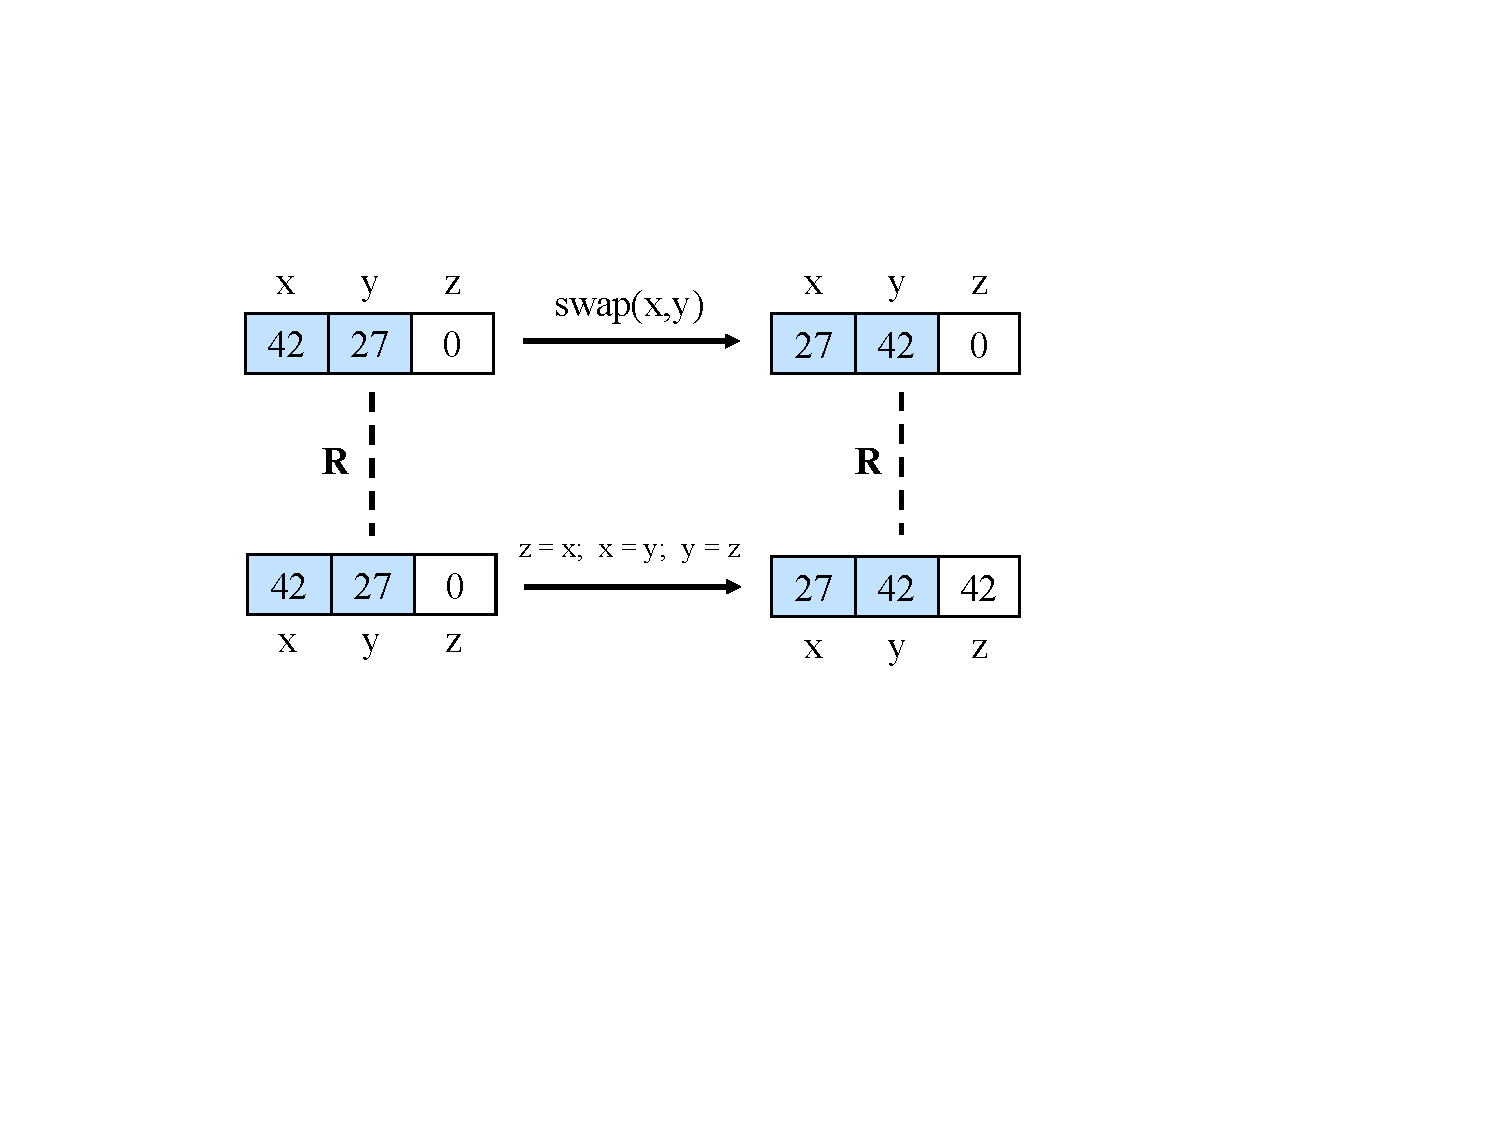
\includegraphics[scale=0.44,origin=c,clip=true,trim=100 220 200 130]{pldi/figure/paradox.pdf}}
\caption{\small{Security-Violating Simulation. The shaded
part of state is unobservable, while the unshaded part is observable.}}
\label{paradox}
\end{figure}

As mentioned above, the root cause of this issue is that there
is some sort of incompatibility between the simulation relation
and the observation function. In particular, security is
formulated in terms of a state indistinguishability relation, but 
the simulation relation may fail to preserve indistinguishability. 
Indeed, for the example of Figure~\ref{paradox}, it is easy to 
demonstrate two indistinguishable program states that are related
by $R$ to two distinguishable ones (since $R$ allows arbitrary change 
in the observable variable $z$). Thus our solution to this 
issue is to restrict simulations to require that state 
indistinguishability is preserved. More formally, given a principal
$p$, in order to show that machine $m$ simulates $M$ under 
simulation relation $R$, the following property must be proved 
for all states $\sigma_1$, $\sigma_2$ of $M$, and
states $s_1$, $s_2$ of $m$:
{\small
\begin{align*}
& \observem{M}{p}{\sigma_1} = \observem{M}{p}{\sigma_2} \land
(\sigma_1,s_1) \in R \land (\sigma_2,s_2) \in R \\
& \qquad \Longrightarrow
\observem{m}{p}{s_1} = \observem{m}{p}{s_2}
\end{align*}}%

